%
% 1-potenzreihen.tex -- Potenzreihenentwicklung holomorpher Funktionen
%
% (c) 2025 Prof Dr Andreas Müller
%
\section{Potenzreihen holomorpher Funktionen
\label{buch:analytisch:section:potenzreihen}}
\kopfrechts{Potenzreihen holomorpher Funktionen}
Konvergente Potenzreihen einer komplexen Variable sind holomorphe
Funktionen.
Da Potenzreihen gliedweise abgeleitet und integriert werden können,
vereinfachen Aussagen über Ableitungen und Stammfunktionen.
Es stellt sich damit die Frage, welche holomorphe Funktionen
eine konvergente Potenzreihe haben.
Wir geben daher der Eigenschaft, eine konvergente Potenzreihe zu haben,
einen Namen.

\begin{definition}[analytisch]
Eine komplexe Funktion $f(z)$ heisst im Punkt $z_0$ \emph{analytisch},
wenn sie eine konvergente Potenzreihen im Punkt $z_0$ besitzt.
\index{analytisch}%
Eine reelle Funktion $f(x)$ heisst im Punkt $x_0$ \emph{reell analytisch},
wenn sie eine konvergente, reelle Potenzreihenentwicklung im Punkt $x_0$
besitzt.
\index{reell analytisch}%
\end{definition}

Die Frage, welche holomorphe Funktionen auch analytisch sind, wird
in diesem Abschnitt geklärt.
Es ist klar, dass Polynome analytisch sind, Polynome sind endliche 
Potenzreihen.
Mit der geometrische Reihe können auch rationale Funktion allein durch
algebraische Operationen in Potenzreihen entwickelt werden, dies wird
in den Abschnitten 
\ref{buch:analytisch:potenzreihen:subsection:geometrisch}
und
\ref{buch:analytisch:potenzreihen:subsection:rational}
durchgeführt.

Der cauchysche Integralsatz stellt einen Zusammenhang zwischen $f(z)$
und den Werten von $f(x)/(x-z)$ auf einem geschlossenen Weg um den
Punkt $z$ her.
Der Nenner kann mit Hilfe der geometrischen Reihe in eine Potenzreihe
verwandelt werden, die sich zu einer Potenzreihe von $f(z)$ umformen
lässt, dies ist das Thema von Abschnitt
\ref{buch:analytisch:potenzreihen:subsection:analytisch}.

%
% 11-polynome.tex -- Potenzreihen von Polynomen
%
% (c) 2026 Prof Dr Andreas Müller
%
\subsection{Potenzreihen von Polynomen
\label{buch:analytisch:potenzreihen:subsection:polynome}}
Das Polynom
\[
p(z)
=
p_0
+ 
p_1z
+
p_2z^2
+
\dots
+
p_{n-1}z^{n-1}
+
p_nz^n
=
\sum_{k=0}^n p_kz^k
\]
ist eine Potenzreihe, die bereits nach endlich vielen Termen
abbricht.
\index{Polynom}%
Wir möchten den Zusammenhang zwischen den Koeffizienten $p_k$
und der Taylor-Reihe von $p(z)$ herstellen.
\index{Taylor-Reihe}%
\index{Potenzreihe}
Dazu benötigen wir eine Formel für die $k$-te Ableitung einer
Potenzfunktion, die wir im folgenden Lemma aus der Produktregel
ableiten.

\begin{lemma}
\label{buch:analytisch:potenzreihen:lemma:ableitung}
Die $k$-te Ableitung von $z^n$ ist
\begin{equation}
\frac{d^k}{dz^k}
z^n
=
\underbrace{
n(n-1)\cdots(n-k+1)
}_{\textstyle\text{$k$ Faktoren}}
z^{n-k}.
\label{buch:analytisch:potenzreihen:eqn:ableitung}
\end{equation}
\end{lemma}

\begin{proof}
Wir beweisen die Formel
\eqref{buch:analytisch:potenzreihen:eqn:ableitung}
durch vollständige Induktion.
Für $k=0$ wird gar nicht abgeleitet, die Formel gilt trivialerweise.

Für den Induktionsschritt nehmen wir jetzt an, dass die Formel für die
$k$-te Ableitung bereits bewiesen ist, und zeigen kann, dass sie auch
für die $(k+1)$-te Ableitung gilt.
Dazu berechnen wir
\begin{align*}
\frac{d^{k+1}}{dz^{k+1}} z^n
&=
\frac{d}{dz}
\frac{d^k}{dz^k}
z^n
\\
&=
\frac{d}{dz}
n(n-1)\dots(n-k+1) z^{n-k}
\\
&=
n(n-1)\dots(n-k+1)(n-k) z^{n-k-1}
\\
&=
n(n-1)\dots(n-k+1)(n-(k+1)+1) z^{n-(k+1)}.
\end{align*}
Dies ist die Formel für die $(k+1)$-te Ableitung.
Damit ist der Induktionsschritt gelungen und damit die Formel
bewiesen.
\end{proof}

Das Polynom $p(z)$ kann auch als Potenzreihe im Punkt $z_0$
geschrieben werden.
Dies kann auf zwei Arten erreicht werden.
Einerseits gilt die Taylor-Reihe
\begin{align*}
p(z)
&=
\sum_{u=0}^n
\frac{1}{u!}
\frac{d^up}{dz^u}(z_0)
(z-z_0)^u.
\intertext{Andererseits kann man eine Potenzreihenentwicklung durch eine
algebraische Umformung erhalten.
Zunächst wendet man auf}
p(z)
&=
p\bigl((z-z_0) + z_0\bigr)
=
\sum_{k=0}^n p_k \bigl((z-z_0)+z_0\bigr)^k
\intertext{die binomische Formel an und erhält}
&=
\sum_{k=0}^n
p_k
\sum_{u+v=k}
\binom{k}{u}
(z-z_0)^u
z_0^v.
\intertext{Durch Umstellung der Summe und Expansion des
Binomialkoeffizienten kann man dies in dir Form}
&=
\sum_{u=0}^n
\Biggl(
\sum_{k=u}^n
p_k
\binom{k}{u}
z_0^{k-u}
\Biggr)
(z-z_0)^u
\\
&=
\sum_{u=0}^n
\Biggl(
\sum_{k=u}^n
p_k
\frac{k(k-1)\cdots(k-u+1)}{u!}
z_0^{k-u}
\Biggr)
(z-z_0)^u
\intertext{bringen.
Der Nenner $u!$ kann aus der inneren Summe herausgezogen werden und
die verbleibenden Terme können mit Hilfe der Formel
\eqref{buch:analytisch:potenzreihen:eqn:ableitung}
in die Form}
&=
\sum_{u=0}^n
\frac{1}{u!}
\Biggl(
\sum_{k=u}^n
p_k
k(k-1)\cdots(k-u+1)
z_0^{k-u}
\Biggr)
(z-z_0)^u
\\
&=
\sum_{u=0}^n
\frac{1}{u!}
\Biggl(
\sum_{k=u}^n
p_k
\frac{d^u}{dz_0^u}z_0^k
\Biggr)
(z-z_0)^u
\intertext{gebracht werden.
Die Ableitung kann aus der inneren Summe herausgezogen werden,
so dass sich die Ableitung}
&=
\sum_{u=0}^n
\frac{1}{u!}
\frac{d^u}{dz_0^u}
\Biggl(
\sum_{k=0}^n
p_k
z_0^k
\Biggr)
(z-z_0)^u
\\
&=
\sum_{u=0}^n
\frac{1}{u!}
\frac{d^up}{dz_0^u}
(z_0)
(z-z_0)^u
\end{align*}
des Polnoms $p(z_0)$ an der Stelle $z_0$ ergibt.
Die algebraisch gefundene Potenzreihe stimmt also automatisch
mit der Taylor-Reihe überein.

%
% 12-geometrisch.tex -- Die geometrische Reihe
%
% (c) 2026 Prof Dr Andreas Müller
%
\subsection{Die geometrische Reihe
\label{buch:analytisch:potenzreihen:subsection:geometrisch}}
Die geometrische Reihe ist die Reihe
\index{geometrische Reihe}%
\[
a+aq+aq^2 + \dots = \sum_{k=0}^\infty aq^k.
\]
Es ist wohlbekannt, dass diese Reihe für $q<1$ konvergent ist und
die Summe
\[
\sum_{k=0}^n aq^k
=
a\frac{q^{n+1}-1}{q-1}
\qquad\Rightarrow\qquad
\sum_{k=0}^n aq^k
=
\lim_{n\to\infty}
a\frac{q^{n+1}-1}{q-1}
=
a\frac{1}{1-q}
\]
hat.

Für komplexe Zahlen $z\in\mathbb{C}$ mit $|z|<1$ definiert die
geometrische Reihe die holomorphe Funktion
\[
\sum_{k=1} z^k
=
\frac{1}{1-z}
=
f(z).
\]
Der Konvergenzradius der Reihe ist $\varrho=1$.
\index{Konvergenzradius}%
Die Polstelle bei $z=1$ führt zu einer divergenten Potenzreihe.
\index{Polstelle}%
\index{divergent}%

Die Funktion 
\begin{equation}
z
\mapsto
\frac{1}{x-z\mathstrut}
\label{buch:analytisch:eqn:1xz}
\end{equation}
ist ebenfalls holomorph, wir möchten sie jetzt in eine im Punkt $a$
zentrierte Potenzreihe entwickeln.
Dazu verwenden wir die Identität
\begin{equation}
\frac{1}{x-z\mathstrut}
=
\frac{1}{(x-a)-(z-a)\mathstrut}
=
\frac{1}{\displaystyle(x-a)\biggl(1-\frac{z-a\mathstrut}{x-a\mathstrut}\biggr)}
=
\frac{1}{x-a}
\cdot
\frac{1}{\displaystyle1-\frac{z-a\mathstrut}{x-a\mathstrut}}.
\label{buch:analytisch:eqn:geometrisch1}
\end{equation}
Der letzte Faktor auf der rechten Seite lässt sich mit der geometrischen
Reihe als Potenzreihe der Form
\begin{equation}
\frac{1}{\displaystyle1-\frac{z-a\mathstrut}{x-a\mathstrut}}
=
\sum_{k=0}^\infty \biggl(\frac{z-a\mathstrut}{x-a\mathstrut}\biggr)^k
=
\sum_{k=0}^\infty
c_k
(z-a)^k
\qquad\text{mit $c_k=1/(x-a)^k$}
\label{buch:analytisch:eqn:geometrischintegriert}
\end{equation}
entwickeln.

%
% 16-rational.tex -- 
%
% (c) 2026 Prof Dr Andreas Müller
%
\subsection{Rationale Funktionen
\label{buch:analytisch:potenzreihen:subsection:rational}}
Eine rationale Funktion ist ein Quotient der Form
\begin{equation}
f(z)
=
\frac{p(z)}{q(z)},
\qquad
p(z),q(z)\in\mathbb{C}[z]
\label{buch:analytisch:potenzreihen:bruch}
\end{equation}
von zwei Polynomen in $z$.
Polynome sind holomorphe Funktionen, die in ganz $\mathbb{C}$
definiert sind.
Nach der Quotientenregel ist auch der Quotient $f(z)$ eine holomorphe
Funktion überall dort, wo $q(z)$ nicht verschwindet.
In diesem Abschnitt untersuchen wir, wie sich für eine solche Funktion
eine Potenzreihenentwicklung finden lässt.

%
% Polynomieller und rationaler Teil
%
\subsubsection{Polynomieller und rationaler Teil}
Durch Polynomdivision lässt sich der Bruch
\eqref{buch:analytisch:potenzreihen:bruch}
in ein Polynom $s(z)$ und einen einfacheren Bruch
\[
f(z) = s(z) + \frac{r(z)}{q(z)}
\]
zerlegen.
Der Grad von $r(z)$ ist kleiner als der Grad von $q(z)$.
Das Polynom $s(z)$ ist bereits eine Potenzreihe mit unendlichem
Konvergenzradius, es muss nur noch der rationale Teil $r(z)/q(z)$
als Potenzreihe dargestellt werden.

%
% Partialbrüche
%
\subsubsection{Partialbrüche}
In der Analysis lernt man, dass eine rationale Funktion eine
Partialbruchzerlegung hat.
Sie wird dort für die Integration rationaler Funktionen verwendet und
wird daher im Abschnitt~\ref{buch:ratint:bernoulli:subsection:partialbruch}
im Kapitel~\ref{chapter:ratint} über das Integrationsproblem genauer
aufgearbeitet.
Für eine Faktorisierung
\[
q(z) = (z-\alpha_1)^{n_1}\cdot\ldots\cdot (z-\alpha_k)^{n_k}
\]
in Linearfaktoren kann der Bruch als 
\[
\frac{r(z)}{q(z)}
=
\sum_{k=1}^n\sum_{l=1}^{n_k} \frac{A_k^l}{(z-\alpha_k)^l}
\]
geschrieben werden.
Man muss also nur noch eine Potenzreihendarstellung für jeden
einzelnen Summanden finden. 

Ein Summand mit Nennergrad 1 hat die geometrische Reihe
\begin{align*}
\frac{A}{z-\alpha}
&=
-\frac{A}{\alpha}
\cdot
\frac{1}{\displaystyle 1-\frac{z\mathstrut}{\alpha}}
=
-\frac{A}{\alpha}
\sum_{i=0}^\infty \frac{z^i}{\alpha^i}
\end{align*}
als Potenzreihendarstellung um den Nullpunkt.
Der Konvergenzradius ist $|\alpha|$.
Eine analoge Potenzreihenentwicklung lässt sich auch für jeden beliebigen
anderen Entwicklungspunkt $z_0$ finden, solange $z_0$ keine Nullstelle
von $q(z)$ ist.

Für Nennergrad $l>1$ ist
\[
\frac{A}{(z-\alpha)^l}
=
(-1)^l
\frac{A}{\alpha^l}
\cdot
\raisebox{-6pt}{$\displaystyle
\left(
\raisebox{6pt}{$\displaystyle
\frac{1}{\displaystyle 1-\frac{z\mathstrut}{\alpha}}
$}
\right)^l
$}
=
(-1)^l
\frac{A}{\alpha^l}
\cdot
\biggl(
\sum_{i=0}^\infty \frac{z^i}{\alpha^i}
\biggr)^l.
\]
Das Produkt von Potenzreihen ist wieder eine Potenzreihe, somit
sind auch rationale Funktionen analytisch.
Ausserdem kann die Potenzreihe durch rein algebraische Umformung
gewonnen werden.
Die Tatsache, dass es sich auch um die Taylor-Reihe handelt,
spielt dabei keine Rolle.


%
% 14-integration.tex -- Integration der geometrischen Reihe
%
% (c) 2026 Prof Dr Andreas Müller
%
\subsection{Integration der geometrischen Reihe
\label{buch:analytisch:potenzreihen:subsection:integration}}
Durch Integration der geometrischen Reihe entlang einer Kurve
$\gamma$, die nicht geschlossen zu sein braucht, kann eine auf
dem Bild $\operatorname{im}\gamma = \gamma(I)$
definierte Funktion $g\colon\gamma(I)\to\mathbb{C}$ zu einer
Funktion $f(z)$ erweitert werden, die automatisch im holomorph und
analytisch ist.
Die Situation ist in Abbildung~\ref{buch:analytisch:fig:integral}
dargestellt.

\begin{satz}
Sei $\gamma\colon I\to\mathbb{C}$ eine differenzierbare Kurve und $g$
eine auf dem Bild $\operatorname{im}(\gamma)=\gamma(I)$ definierte 
stetige komplexe Funktion.
Dann ist die auf $\mathbb{C}\setminus\operatorname{im}\gamma$ definierte
Funktion
\begin{equation}
f(z)
=
\frac{1}{2\pi i}
\int_\gamma
\frac{g(x)}{x-z\mathstrut}\,dx
\end{equation}
holomorph.
\end{satz}

\begin{proof}
Da das Integrationsgebiet kompakt ist und $f$ stetig ist, kann unter
dem Integral differenziert werden.
Es ergibt sich die Ableitung
\begin{align*}
f'(z)
&=
\frac{1}{2\pi i}
\frac{d}{dz}
\int_\gamma
\frac{g(x)}{x-z\mathstrut}
\,dx
=
\frac{1}{2\pi i}
\int_\gamma
\frac{d}{dz}
\frac{g(x)}{x-z\mathstrut}
\,dx
=
\frac{1}{2\pi i}
\int_\gamma
\frac{g(x)}{(x-z\mathstrut)^2}
\,dx
\end{align*}
Insbesondere ist $f(z)$ komplex differenzierbar und damit $f$ holomorph.
\end{proof}

Andererseits kann man den Integranden mit der geometrischen Reihe
entwickeln und termweise integrieren.
%
% fig-integral.tex -- Integral der geometrischen Reihe
%
% (c) 2026 Prof Dr Andreas Müller
%
\begin{figure}
\centering
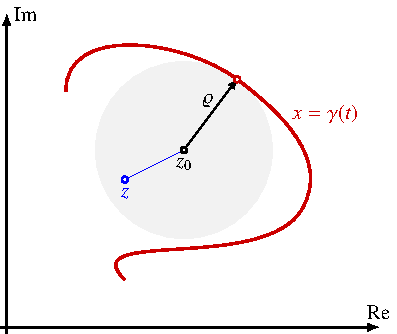
\includegraphics{chapters/040-analytisch/images/integral.pdf}
\caption{Durch Integration der geometrischen Reihe um den Punkte $z_0$
entlang eines nicht notwendigerweise geschlossenen Pfades $\gamma$ 
entsteht aus einer stetigen Funktion $g(x)$ auf der Kurve eine im
Komplement der Kurve holomorphe Funktion $f(z)$.
Um den Punkt $z_0$ kann für $f(z)$ eine eine Potenzreiheentwicklung 
angegeben werden kann, die als Konvergenzradius den minimalen
Abstand $\varrho$ zur Kurve hat.
\label{buch:analytisch:fig:integral}}
\end{figure}
%
Dazu verwenden wir
\eqref{buch:analytisch:eqn:geometrisch1}
und
\eqref{buch:analytisch:eqn:geometrischintegriert}
und erhalten
\begin{align}
f(z)
&=
\frac{1}{2\pi i}
\int_\gamma
\frac{g(x)}{x-z_0}
\cdot
\frac{1}{\displaystyle1-\frac{z-a\mathstrut}{x-a\mathstrut}}
\,dx
\notag
\\
&=
\frac{1}{2\pi i}
\int_\gamma
\frac{g(x)}{x-z_0}
\sum_{k=0}^\infty
\biggl(
\frac{z-z_0\mathstrut}{x-z_0\mathstrut}
\biggr)^k
\,dx
\notag
\\
&=
\sum_{k=0}^\infty
\biggl(
\frac{1}{2\pi i}
\int_\gamma
\frac{g(x)}{(x-z_0)^{k+1}}
\,dx
\biggr)
(z-z_0)^k.
\label{buch:analytisch:eqn:reihe}
\end{align}
Damit ist eine Potenzreihe im Punkt $a$ für die Funktion
$f(z)$ gefunden.
Sie ist konvergent, solange 
\[
\biggl|
\frac{z-z_0}{x-z_0}
\biggr|
=
\frac{|z-z_0|}{|x-z_0|}
<
1
\qquad\Rightarrow\qquad
|z-z_0| < |x-z_0|
\]
für alle $x$ entlang des Weges $\gamma$ gilt.
Dies wird erreicht, wenn 
\[
|z-z_0| < \inf_{\gamma} |x-z_0|,
\]
auf der rechten Seite steht der kleinste Abstand des Punktes $a$ vom
Weg $\gamma$.
Wir fassen dieses Resultat im folgenden Satz zusammen.

\begin{satz}
\label{buch:analytisch:potenzreihen:satz:integralanalytisch}
Sei $\gamma\colon I\to\mathbb{C}$ eine Kurve in $\mathbb{C}$ und
$f$ eine stetige Funktion auf dem Bild $\gamma(I)=\operatorname{im}\gamma$
der Kurve.
Dann ist die Funktion 
\begin{equation}
f(z)
=
\int_{\gamma} \frac{g(x)}{x-z}\,dx
\label{buch:analytisch:potenzreihen:eqn:fzintegral}
\end{equation}
analytisch und hat im Punkt $z_0 \in\mathbb{C}\setminus \operatorname{im}\gamma$
die Potenzreihenentwicklung
\[
f(z)
=
\sum_{k=0}^\infty
\biggl(
\frac1{2\pi i}
\int_\gamma \frac{g(x)}{(x-z_0)^{k+1}}\,dx
\biggr)
(z-z_0)^k
\]
mit Konvergenzradius
\[
\varrho(z_0)
=
\inf\{ |\gamma(t)-z_0|\mid t\in I\}.
\]
\end{satz}

%
% 15-analytisch.tex -- Potenzreihenentwicklung einer holomorphen Funktion
%
% (c) 2026 Prof Dr Andreas Müller
%
\subsection{Potenzreihenentwicklung einer holomorphen Funktion
\label{buch:analytisch:potenzreihen:subsection:analytisch}}
Falls für eine komplexe Funktion eine konvergente Potenzreihenentwicklung
existiert, dann ist die Funktion sogar unendlich oft stetig differenzierbar.
Ob auch die Umkehrung gilt, wissen wir noch nicht.
Die Existenz einer konvergenten Potenzreihe und die Existenz einer
komplexen Ableitung sind also nach unserem aktuellen Wissensstand
nicht notwendigerweise dasselbe.

Wir wissen aber nach
Satz~\ref{buch:analytisch:potenzreihen:satz:integralanalytisch},
dass eine holomorphe Funktion, die durch das
Integral~\eqref{buch:analytisch:potenzreihen:eqn:fzintegral}
aus den Werten einer stetigen Funktion entlang einer Kurve
entsteht, analytisch ist.
Wir können diese Erkenntnis nun mit dem cauchyschen Integralsatz
zusammenbringen und zeigen, dass jede holomorphe Funktion auch
eine konvergente Potenzreihenentwicklung hat.

Sei jetzt also $f(z)$ eine holomorphe Funktion und $\gamma$ ein
geschlossener Weg, der ein Gebiet $U$ berandet und genau einmal
umläuft.
Satz~\ref{buch:analytisch:potenzreihen:satz:integralanalytisch}
sagt für $g(x)=f(z)$, dass das
Integral~\eqref{buch:analytisch:potenzreihen:eqn:fzintegral}
eine analytische Funktion ist.
Der cauchysche Integralsatz sagt andererseits, dass sie in $U$ mit
$f(z)$ übereinstimmt.
Damit haben wir den folgenden Satz gezeigt.

\begin{satz}[holomorphe Funktionen sind analytisch]
\label{buch:analytisch:satz:holomorph-analytisch}
Eine holomorphe Funktion $f(z)$ ist analytisch, die Taylor-Reihe
von $f$ im Punkt $a$ konvergiert.
Der Konvergenzradius ist das Supremum der Radien von Kreisen um $a$,
die vollständig im Definitionsbereich von $f$ enthalten sind.
\end{satz}

Die Integrale auf der rechten Seite von \eqref{buch:analytisch:eqn:reihe}
können ebenfalls mit dem Satz~\ref{buch:integration:satz:ableitungn}
ausgerechnet werden.
Wegen
\[
f^{(k)}(z)
=
\frac{k!}{2\pi i}
\oint_\gamma
\frac{f(x)}{(x-z)^{k+1}}
\,dx
\]
ergeben sie
\begin{align*}
f(z)
&=
\sum_{k=0}^{\infty}
\biggl(
\frac{1}{2\pi i}
\oint_\gamma
\frac{f(x)}
{(x-z_0)^{k+1}}
\,dx
\biggr)
(z-z_0)^k
=
\sum_{k=0}^\infty
\frac{f^{(k)}(z_0)}{k!}
(z-z_0)^k.
\end{align*}
Damit ist die gefundene Potenzreihe der Funktion $f$ die
Taylor-Reihe der Funktion $f$ im Punkt $z_0$.

Der Satz~\ref{buch:analytisch:satz:holomorph-analytisch}
hat gezeigt, dass eine holomorphe Funktion immer auch
analytisch ist.
Dies ist eine Eigenschaft, die nicht für reelle analytische
Funktionen gilt, wie im nachfolgenden Abschnitt gezeigt wird.

%
% 16-reellanalytisch.tex -- Reelle differenzierbare Funktionen sind nicht alle analytisch
%
% (c) 2026 Prof Dr Andreas Müller
%
\subsection{Reelle differenzerierbare Funktionen sind nicht alle analytisch}
Die Aussage des Satzes~\ref{buch:analytisch:satz:holomorph-analytisch}
hat keine Entsprechung für reelle beliebig oft differenzierbare
Funktionen.
Vielmehr gibt es beliebig oft differenzierbare reellwertige
Funktionen auf $\mathbb{R}$, die keine konvergente Potenzreihe haben.
Wir konstruieren in diesem Abschnitt ein solches Beispiel.

%
% Eine glatte Funktion mit verschwindender Potenzreihe
%
\subsubsection{Eine glatte Funktion mit verschwindender Potenzreihe}
\input{chapters/040-analytisch/fig/fig-nichtanalytisch.tex}%
Wir betrachten die Funktion
\begin{equation}
f(x)
=
\begin{cases}
e^{-1/x}&\qquad \text{für $x>0$}\\
0&\qquad\text{sonst}
\end{cases}
\label{buch:analytisch:fig:nichtanalytisch}
\end{equation}
(siehe auch Abbildung~\ref{buch:analytisch:fig:nichtanalytisch}).
Sie ist beliebig oft differenzierbar.
Die Ableitung ist ausserhalb des Punktes $x=0$ stetig, es muss also
nur noch untersucht werden, dass die Ableitung auch im Punkt $x=0$
stetig ist.

%
% Die Ableitungen von e^{-1/x} im Punkt 0
%
\subsubsection{Die Ableitungen von $e^{-1/x}$ im Punkt $0$}
Die Ableitung von $f(x)$ ist
\begin{equation}
f'(x)
=
\frac{1}{x^2}
e^{-1/x}
\label{buch:analytisch:eqn:f'}
\end{equation}
für $x>0$.
Für höhere Ableitungen wird der Ausdruck komplizierter, wir wollen
mit vollständiger Induktion zeigen, dass alle Ableitungen von der Form
\begin{equation}
f^{(n)}(x)
=
P_n\biggl(\frac1x\biggr) e^{-1/x}
\label{buch:analytisch:eqn:fn=Pne}
\end{equation}
ist, wobei $P_n$ ein Polynom ist.
Die Gleichung \eqref{buch:analytisch:eqn:f'} dient dazu als
Induktionsverankerung.

Für den Induktionsschritt nehmen wir jetzt an, dass 
\eqref{buch:analytisch:eqn:fn=Pne}
für die $n$-te Ableitung gilt und zeigen, dass auch die $n+1$-te
Ableitung diese Form hat.
Dazu berechnen wir
\begin{align*}
f^{(n+1)}(x)
&=
\frac{d}{dx}
f^{(n)}(x)
=
\frac{d}{dx} P\biggl(\frac1x\biggr) e^{-1/x}
\\
&=
-P'_n\biggl(\frac1x\biggr) \frac{1}{x^2} e^{-1/x}
+
P_n\biggl(\frac1x\biggr) \frac{1}{x^2} e^{-1/x}
\\
&=
\frac{1}{x^2}
\biggl(
P_n\biggl(\frac1x\biggr)
-
P_n'\biggl(\frac1x\biggr)
\biggr)e^{-1/x}
\end{align*}
Setzt man 
\begin{equation}
P_{n+1}(X)
=
X^2(P_n(X) - P'_n(X)),
\label{buch:analytisch:eqn:e1rekursion}
\end{equation}
kann man tatsächlich
\[
f^{(n+1)}(x)
=
P_{n+1}\biggl(\frac1x\biggr)e^{-1/x}
\]
schreiben.
Die Rekursionsformel~\eqref{buch:analytisch:eqn:e1rekursion}
liefert ein Polynom $P_{n+1}$, womit der Induktionsschritt vollzogen
ist.

Die Polynome $P_n$ aus dem vorangegangenen Beweis lassen sich
mit der Rekursionsformel~\eqref{buch:analytisch:eqn:e1rekursion}
sehr leicht berechnen, die ersten paar Polynome sind
\begin{align*}
P_0(X) &= 1 \\
P_1(X) &= X^2 \\
P_2(X) &= X^4 - 2X^3 \\
P_3(X) &= X^2 (X^4 - 2X^3 - 4X^3 + 6X^2) = X^6 -6X^5+6X^4 \\
P_4(X) &= X^8 -12X^7+36X^6-24X^5 \\
P_5(X) &= X^{10} -20X^9 +120 X^8 - 240X^7 + 120 X^6.
\end{align*}
Da für $x\to 0$ der Exponentialfaktor $e^{-1/x}$ immer schneller
gegen $0$ geht, als ein polynomialer Faktor $P_n(1/x)$ gegen $\infty$
gehen kann, ist der Grenzwert 
\[
\lim_{x\to 0+}
f^{(n)}(x)
=
\lim_{\xi\to \infty}
P_n(\xi) e^{-\xi}
=
0.
\]
Damit ist gezeigt, dass an der Stelle $x=0$ alle Ableitungen von $f$
stetig sind, $f$ ist eine glatte Funktion.

Da die Ableitungen an der Stelle $x=0$ verschwinden, ist die
Taylor-Reihe von $f$ die Nullfunktion.
Da $f$ selbst nicht die Nullfunktion ist, kann die Taylor-Reihe
nicht gegen $f$ konvergieren.
%
% Die Funktion f(x) ist nicht Einschränkung einer holomorphen Funktion
%
\subsubsection{Die Funktion $f(x)$ ist nicht Einschränkung einer holomorphen Funktion}
Die Funktion $f(x)$ lässt sich nicht zu einer holomorphen Funktion
ausdehnen.
Der einzige dafür in Frage kommende Kandidat ist die Funktion
$z\mapsto e^{-1/z}$.
Nähert sich $z$ auf der imaginären Achse dem Punkt $0$, zum Beispiel
mit $z=i/t$ für $t\to \infty$, dann ist
\[
\lim_{\varepsilon\to 0} e^{-1/i\varepsilon}
=
\lim_{t\to\infty} e^{it}
=
\lim_{t\to\infty}(\cos t + i\sin t).
\]
Der Grenzwert auf der rechten Seite konvergiert allerdings nicht, sodass
die Funktion $z\mapsto e^{-1/z}$ im Punkt $z=0$ nicht einmal stetig
sein kann.


